\chapter{Experiments} % (fold)
\label{cha:experimental_setup}

The theory on local exemplar-NBNN detection was tested in a number of experiments. First, the NBNN detection experiments of Becker \emph{et al.} \cite{becker2012codebook} were replicated to validate the implementation, see Section~\ref{sec:nbnn_detection}. These experiments were altered in a number of ways, to see the effects of different clustering algorithms and descriptor detection methods. Next to this, exemplar-$k$NBNN was tested, both with and without McCann's Local NBNN approach (Section~\ref{sec:local_nbnn_detection}). Most tests were performed on both the TUD motorbikes and VOC 2007 benchmark detection sets.

\section{Features} % (fold)
\label{sec:features}

In most experiments, feature detection is done by dense sampling. Each point was sampled at various scales, to allow for scale invariance. The descriptor that has been used was the scale-invariant feature transform (SIFT) \cite{lowe2004distinctive}.

For some experiments, SIFT features were detected using Harris-Laplacian interest point detection \cite{mikolajczyk2005comparison, vandeSande2010colorSIFT}. This detector finds potential interest points based on Harris corner detection, and then selects the most appropriate scale for each by finding a maximum over a Laplacian-of-Gaussians. The SIFT features are taken at these locations and at these scales. Compared to dense sampling, interest point detection gets relatively few features, but rather distinctive ones. Boiman claims dense sampling is necessary for NBNN (\emph{cf.} Section~\ref{cha:naive_bayes_nearest_neighbor}), but its performance/efficiency tradeoff for exemplar-NBNN detection might be different.

% section features (end)

\section{PASCAL VOC Data Set} % (fold)

\label{sec:voc_data_set}
The Visual Object Classes (VOC) 2007 challenge of the PASCAL network \cite{pascal-voc-2007} provides a data set annotated for image detection. The data set consists of 20 object classes plus a background class, on a total of 9,963 images containing 24,640 annotated objects. The images are all taken from Flickr, and show a large variety of image quality and a large intra-class variety of objects. The data set is subdivided into 50\% test set, 25\% training set and 25\% validation set, with an approximately equal distribution of class object distribution over the sets.

The VOC 2007 dataset is partly annotated for class segmentation consisting of 632 images subdivided into 210 test images, 213 validation images and 209 train images, approximately equally distributed over the classes. For the experiments below, the combined segmentation training and validation sets (422 images) were used to train. The main reason for this training set is that segmentation proved to be a good ground truth for class assignment of features. On top of that, the full VOC 2007 training set appeared prone to exceed time and memory constraints. Testing was done both on the segmentation test set and the full test set.

For performance comparison the results of the Pascal VOC 2007 detection challenge were used. For each class, the score of the best performing contender was taken and this provided the baseline scores. These scores give a good measure of the state-of-the-art at the time. While being outdated, it gives good comparison material for the new results.

% section voc_data_set (end)

\section{TUD Motorbikes Data Set} % (fold)
\label{sec:tudmotorbikes_data_set}
The TUD Motorbikes data set is a selection of motorbikes from different benchmark sets. \cite{fritz2005integrating} The training set consists of 153 images of motorbikes on a uniform background, and are segmented into 2 classes: \emph{motorbike} and \emph{background}. The test set consists of 115 images, all of motorbikes, with various background, and ground truth bounding boxes. Becker \emph{et al.} \cite{becker2012codebook} use this benchmark to test their setup. In the training phase they train on the motorbike features from the TUD train set, and they add features from non-object areas of 300 random images of the PASCAL VOC 2007 set, as background features.

This same setup was used here, as a comparison to Becker's experiments. Even though this was not reported by Becker, I decided to perform the experiments on the TUD set in 5-fold, each time with a different randomized set of background images, but using the same sets when running the various experiments to keep the results as much comparable as possible. Results of the experiments were compared to the performance of Becker, who got an average precision of 83.20\%, and an equal error rate of 84.1\%.

% section tudmotorbikes_data_set (end)


% SKIP THIS PART
% \section{NBNN Classification} % (fold)
% \label{sec:nbnn-cls}
% \todo[inline,color=red]{This section only if the tests succeed. Most of the method is already in the NBNN section.}
% 
% % section nbnn-cls (end)

\section{Exemplar-NBNN Detection} % (fold)
\label{sec:nbnn_detection}

The first experiment is used to verify the results of Becker \emph{et al.} \cite{becker2012codebook}. In addition to this, some parameters of this approach were altered to see what effects they have on the overall performance.

This experiment was performed on the TUD Motorbike set in the setup used by Becker (cf. Section~\ref{sec:tudmotorbikes_data_set}). The SIFT descriptors were collected with dense sampling, using a step size of 8 pixels, and patch sizes of $32\times32$, $48\times48$ and $64\times64$. I repeated each test 5 times with a different random selection of background images from the VOC 2007 data set, to avoid possible artifacts. FLANN was used to perform approximate NN, using the kd-tree algorithm with 4 trees and 1000 checks to assure high enough accuracy.

The similarity measure between hypotheses, used as a basis for the clustering algorithm, was defined as the area of overlap ($AO$) between two hypotheses:
\begin{equation}
    AO(H_a, H_b)= \frac{|H_a\cap H_b|}{|H_a\cup H_b|}
\end{equation}

Clustering was done using the single-link agglomerative clustering algorithm (Section~\ref{sub:agglomerative_clustering}), using 2 parameters: $\theta_m$, which defines the minimal overlap between hypotheses to be clustered together, and the maximal overlap between detections: $\theta_p$. I set the parameters such that $\theta_m = 0.8$ and $\theta_p = 0$, to conform with Becker.

Detections were ranked according to their ``detection quality'', $Q_D$. This measure is defined as the amount of hypotheses being clustered into one detection. Ties being broken by a second ordering, called ``hypothesis quality'', $Q_H$, which is defined in Equation~\eqref{eq:qh}. Performance was measured with the average precision (AP) of the ranked detections, and visualized in a precision-recall curve.

\subsection{NBNN Detection Using Quickshift clustering} % (fold)
\label{sub:nbnn_detection_using_quickshift_clustering}

The results of detection using single link clustering were compared to quickshift clustering. Quickshift has one parameter, $\tau$. This represents the expected variance within the clustering space, and defines the maximal variance to be clustered, somewhat like $\theta_m$ in single link clustering.

Quickshift has no bound for overlap in detections, which should not be a problem as the test images might have multiple overlapping objects. To make this comparison fair towards single link clustering, I varied the value of $\theta_p$ in the latter algorithm. For quickshift I settled on $\tau = 1.2$, for single link clustering $\theta_p = 0.4$ seemed ideal.

% subsection nbnn_detection_using_quickshift_clustering (end)
% \subsection{Training Weighted Distances} % (fold)
% \label{ssub:training_weighted_distances}
% 
% In image classification, the classes are generally quite well balanced. The amount of images in every class is usually approximately the same and all image are usually of the same size, making the assumption of a uniform prior hold. Therefore the natural distribution of descriptors in feature-space can be assumed to be equally sampled in every class. This makes it acceptable to use a learning method like optimal NBNN \cite{behmo2010towards} to tune the likelihood of classes to the local density in feature space to be equal for all classes.
% 
% In object detection, the sampling rate will not be equal over classes, especially the background class will have a larger sampling rate, simply because it will occur in virtually all images. The equal priors assumption therefore does not hold. This flaw is mitigated by the fact that a higher number of sampled descriptors also tends to make the feature space for that class more dense, and more likely to be the nearest neighbor.
% 
% The risk however is that the estimation of the feature space may differ largely per class. Classes with a large intra-class variety of descriptors, but with generally small objects will be sampled much sparser than classes with less descriptor variety and larger objects. Learning parameters to tune the feature space density might therefore result in overfitting for sparsely sampled classes or classes with a very high intra-class diversity.
% 
% This experiment will test this hypothesis using Behmo's optimal NBNN linear program to train per-class parameters on sampled images.
% 
% \todo[inline]{more detail about implementation of Behmo. Perhaps put the first part either to conclusion, or to theory?}

% subsubsection training_weighted_distances (end)

\subsection{Exemplar-NBNN Results} % (fold)
\label{sub:exemplar_nbnn_results}
% k=1:
% 
% On TUD:
% \begin{itemize}
%     \item Becker original reported baseline
%     \item Own Becker implementation: k=1,SL0
%     \item Quickshift, k=1, 1.2
%     \item SL, k=1, 0.4
%     \item Harrislaplacian QS1.2, k=1
%     \item Behmo???
% \end{itemize}
% 
% On VOC:
% \begin{itemize}
%     \item Becker implemtnation dsift,k=1,SL0 (have FULLTEST TOO)
%     \item DUPLICATE dsift,k=1,SL0
%     \item dsift,sl4,k=1
%     \item dsift, qs1.2,k=1
%     \item hlp, qs1.2, k=1 RUNNNING
% \end{itemize}
% 
% nonlocal k>1:
% TUD:
% \begin{itemize}
%     \item Becker, dsift,k=20,SL0 (dont have it)
%     \item dsift,k=20,SL4
%     \item dsift, k=4,qs12
%     \item hlp, k=4, qs12
% \end{itemize}
% 
% VOC:
% \begin{itemize}
%     \item dsift, k=4,qs12
%     \item hlpsift,k=4,qs12
% \end{itemize}
% 
% Local k>1:
% TUD:
% \begin{itemize}
%     \item dsift, k=20,SL4
%     \item dsift, k=4, qs12 (???)
%     \item hlp, k=4, qs12
% \end{itemize}
% 
% VOC:
% \begin{itemize}
%     \item dsift, k=4, qs12
%     \item hlp, k=4, qs12 (have FULLTEST TOO)
% \end{itemize}
% 
% 
% VOC FULLTEST:
% \begin{itemize}
%     \item Becker implemtnation dsift,k=1,SL0
%     \item local: hlp, k=4, qs12
% \end{itemize}

Figure~\ref{fig:tudk1prc} and Table~\ref{tab:tudallstats} show the results on the TUD set, of the implementation of Becker's algorithm using Single-link clustering compared to the results reported by Becker \cite{becker2012codebook}. It also shows the results using the quickshift algorithm and using single-link clustering with $\theta_p = 0.4$, instead of Becker's $\theta_p = 0.0$. 

Note that I labeled all experiments using their settings mentioning descriptor detection method (``ds'' or ``hl'' for dense sampling and harris-laplace), ``loc'' for LNBNN tests, a value for $k$, and the clustering algorithm: QS, SL$_{0.0}$ and SL$_{0.4}$ for quickshift, single link clustering with $\theta_p=0.0$ and $\theta_p=0.4$ respectively. This way, the reference experiment becomes ``ds, $k_1$,SL$_{0.0}$''. For the VOC 2007 set, the test set was added as either ``st'' or ``ft'', for segmentation test set or full test set.

The results shown in Figure~\ref{fig:tudk1prc} and Table~\ref{tab:tudallstats} show that quickshift performs slightly better than single-link clustering on the TUD test, and that dense sampling is indeed crucial, seeing the major decline in performance when harris-laplacian feature selection was used.

\begin{figure}[hbt]
    \centering
    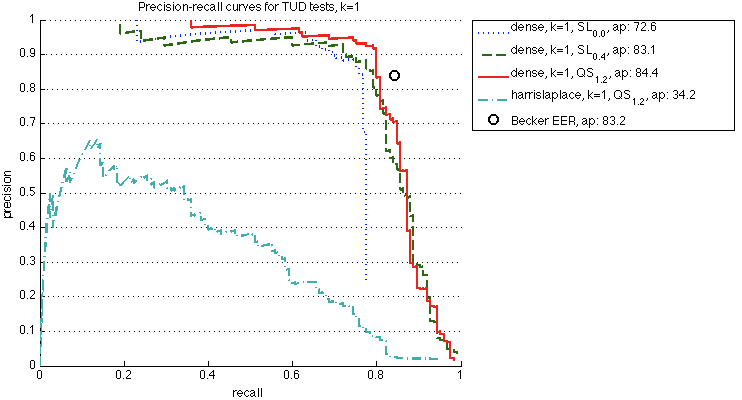
\includegraphics[width=0.9\textwidth]{TUDk1prc}
    \caption{Precision-Recall curves of the TUD Motorbikes detection task. Comparing Becker's \cite{becker2012codebook} setup with various settings, keeping $k=1$. Curves provided are all based on a test using the same random background set (except the reference Equal Error Rate reported by Becker).}
    \label{fig:tudk1prc}
\end{figure}

\begin{table}
    \caption{Comparison of test statistics of TUD Motorbikes tests using various clustering algorithms and settings. ``Becker Baseline'' represents the result reported by Becker \cite{becker2012codebook}. All other results are averaged over 5 randomized tests.}
    \label{tab:tudallstats}
    \begin{tabular}{r|rrr|c}
    Method&duration (hrs)&max. recall&detections&avg. prec.\\
    Becker Baseline&---&84.50&---&83.20\\
    ds, $k_1$, SL$_{0.0}$&0.34&76.32&390&72.59\\
    ds, $k_1$, SL$_{0.4}$&0.39&99.36&3412&83.14\\
    ds, $k_1$, QS &0.46&99.20&7874&84.38\\
    hl, $k_1$, QS &0.39&94.40&6062&34.21\\
    ds, $k_{20}$, SL$_{0.4}$&2.30&98.56&3673&84.78\\
    ds, $k_4$, QS &1.09&97.76&8189&\underline{87.88}\\
    hl, $k_4$, QS &0.43&94.40&6768&43.57\\
    ds, $k_{20}$, loc, SL$_{0.4}$&87.27&80.80&6997&52.36\\
    hl, $k_4$, loc, QS &0.69&77.60&13052&21.24\\
    ds, $k_4$, loc, QS &7.59&93.60&12467&79.48
    \end{tabular}
\end{table}

The $k=1$ entries of Table~\ref{tab:tudallstats} show some more statistics of the experiments. The results reported by Becker are somewhat higher than my own basic replication. This might be caused by a fortunate set of random background descriptors in the reference test, while my results are averaged over 5 random sets. Becker does not report the randomization process involved, so I was not able to replicate the results exactly. The results clearly show that raising the $\theta_p$ threshold for the maximal overlap between detections is beneficial, mainly because the recall gets higher. It also shows this change raises the total number of detections found by a factor $>10$, quickshift generating more detections than single-link using similar settings. Interestingly, interest point detection seems to generate almost all correct detections with maximal recall of 94\%. The low AP can only be explained by a bad ranking of detections.

\begin{figure}[hbt]
    \centering
    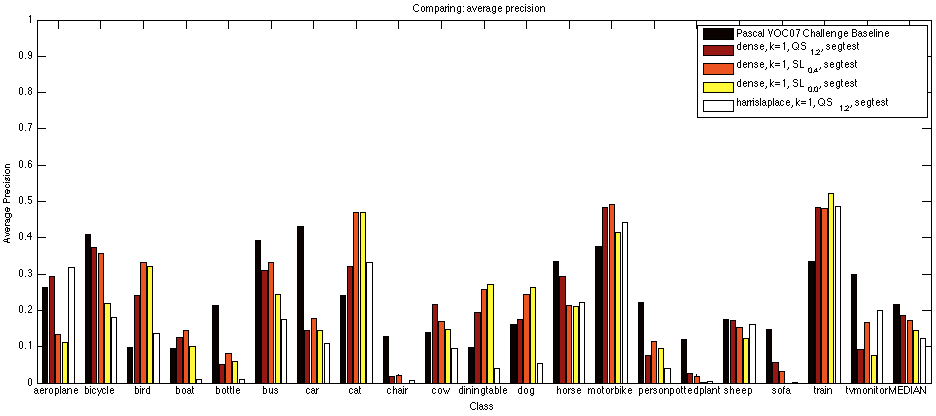
\includegraphics[width=\textwidth]{VOCk1ap}
    \caption{AP for each VOC 2007 class of various tests using $k=1$, sorted by the median of AP over all classes.}
    \label{fig:vock1ap}
\end{figure}

On the VOC 2007 dataset, overall performance is lower than on the TUD set, which was expected. Figure~\ref{fig:vock1ap} and Table~\ref{tab:vocallaps} show that the overall performance of exemplar NBNN (with $k=1$) is lower than that of the baseline. The results however vary greatly over the classes. In 8 classes, the experiment using Becker's settings (``ds, $k_1$, SL$_{0.0}$, st'') gets a higher AP than the baseline. At the same time, some classes get APs which are much lower than the baseline, notably \emph{bottle}, \emph{car}, \emph{chair}, \emph{person}, \emph{pottedplant}, \emph{sofa} and \emph{tvmonitor}. Looking at the median of the APs over all classes, taken as a measure to compare overall performance, it shows that on average the $k=1$ methods perform somewhat less than the baseline. It also confirms the results on the TUD experiments: quickshift seems to perform better than single-link clustering, in single-link clustering overlap between detections should be allowed, and dense sampling gives better performance than interest point detection.

Looking at some other statistics of these VOC experiments in Table~\ref{tab:vocalldurdet}, it shows that interest point detection results in large time savings. Again, the increase of the amount of detections is quite steep as overlap between detections is allowed.

% subsection exemplar_nbnn_results (end)

% section nbnn_detection (end)

\section{Exemplar-$k$NBNN Detection} % (fold)
\label{sec:local_nbnn_detection}
A downside of the exemplar-NBNN method is the descriptor aliasing problem explained in Section~\ref{sec:descriptor_aliasing}. This can be solved by taking the $k$ of $k$NN to be greater than 1. This means that the $k$ closest neighbors over all classes (the object class and the background class) are taken into account when constructing detection hypotheses. Within these $k$ nearest neighbors, the ones belonging to the object class that are closer than any neighbor in the background class, are transformed into detection hypotheses. This $k$NBNN approach was tested in the detection algorithm and compared to the previous setup. 

\subsection{Local NBNN Detection} % (fold)
\label{ssub:local_nbnn_detection}

Another disadvantage of exemplar-NBNN detection is it returning many false positive detections for images not having any objects of the current object class. The reason for this is obvious, as all descriptors closer to the class than to the background will be regarded as hypotheses, and therefore images without any objects get reasonably well ranked detections. This problem gets larger as the data sets contain more object classes.

A solution for this is to not only compare the current object class with the background class, but to compare it with all other classes, to see what each descriptor in the test image looks most like. This results in a hypothesis selection step that chooses only descriptors that are closer to the current class than to any other.

This however would create another problem not present in the original approach. Some descriptors could be an indicator for multiple classes, because certain parts of objects are quite similar. While the original exemplar-NBNN approach allows for this, regarding each class independently, this multi-class approach prevents this. Think of the similarity of a bicycle wheel with that of a motorbike or a car. To disregard all but one of these classes might cause very little evidence for most classes in an image, giving less stable detections. This reminds of Boiman's argument that much evidence is vital for the NBNN method, because the Naive Bayes assumption is only met towards infinity and there is no training phase to compensate for it \cite{boiman2008defense}.

At the same time, the goal to compare all classes simultaneously is similar to McCann \& Lowe's formulation of the LNBNN query. \cite{mccann2012local} (\emph{cf.} Section~\ref{sec:local_nbnn}). Merging all class indexes into one, and taking into account not only the first NN per class, but the \emph{overall} $k$NN prevents having too many false positive results, while keeping the possibility of a descriptor to be used for a hypothesis for multiple classes like in the original problem.

As a bonus, LNBNN detection also incorporates a way to prevent the aliasing problem (\emph{cf.} Section~\ref{sec:descriptor_aliasing}). Among the $k$ closest neighbors, there might be multiple ones from the same class. Instead of disregarding these neighbors like local NBNN does, they can be taken into account by creating hypotheses for all non-background nearest neighbors.

% subsubsection local_nbnn_detection (end)

\subsection{Exemplar $k$NBNN \& LNBNN Results} % (fold)
\label{ssub:lnbnn_results}

\begin{figure}[hbt]
    \centering
    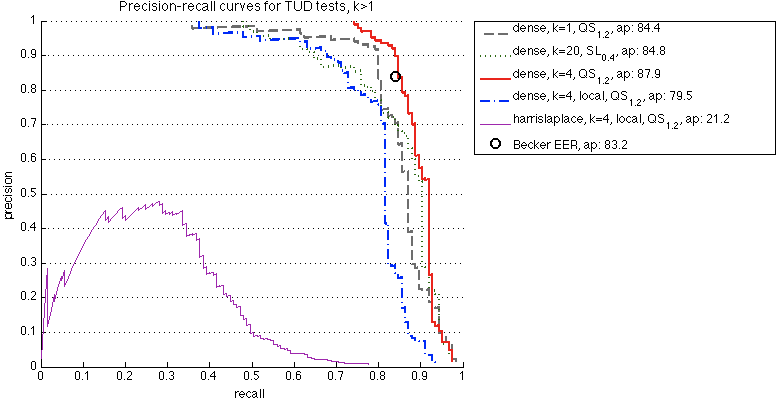
\includegraphics[width=0.9\textwidth]{TUDklocprc}
    \caption{Precision-Recall curves of the TUD Motorbikes detection task, of various tests with $k>1$.}
    \label{fig:tudklocprc}
\end{figure}



As shown in Figure~\ref{fig:tudklocprc} and Table~\ref{tab:tudallstats}, $k$NBNN detection on the TUD task improves average precision compared to 1NBNN. The optimal amount of neighbors appeared to be at $k=4$ for quickshift clustering, while the optimum for single-link runs was at $k=20$. Interestingly, LNBNN seems to perform less well than regular $k$NBNN. This might be due to the task, having only one class and all test images containing at least one motorbike, while LNBNN was built specifically for multiple-class detection and the probability of a class appearing on an image being less than one.

Again, interest point detection harms performances greatly compared to dense sampling, and quickshift always performs better than single-link clustering. Furthermore, the amount of detections seems to get quite big in quickshift-LNBNN experiments. The ``ds, $k_{20}$, loc, SL$_{0.4}$'' experiment took 87 hours, which is extraordinary. This is probably due to a memory issue.

\begin{figure}[hbt]
    \centering
    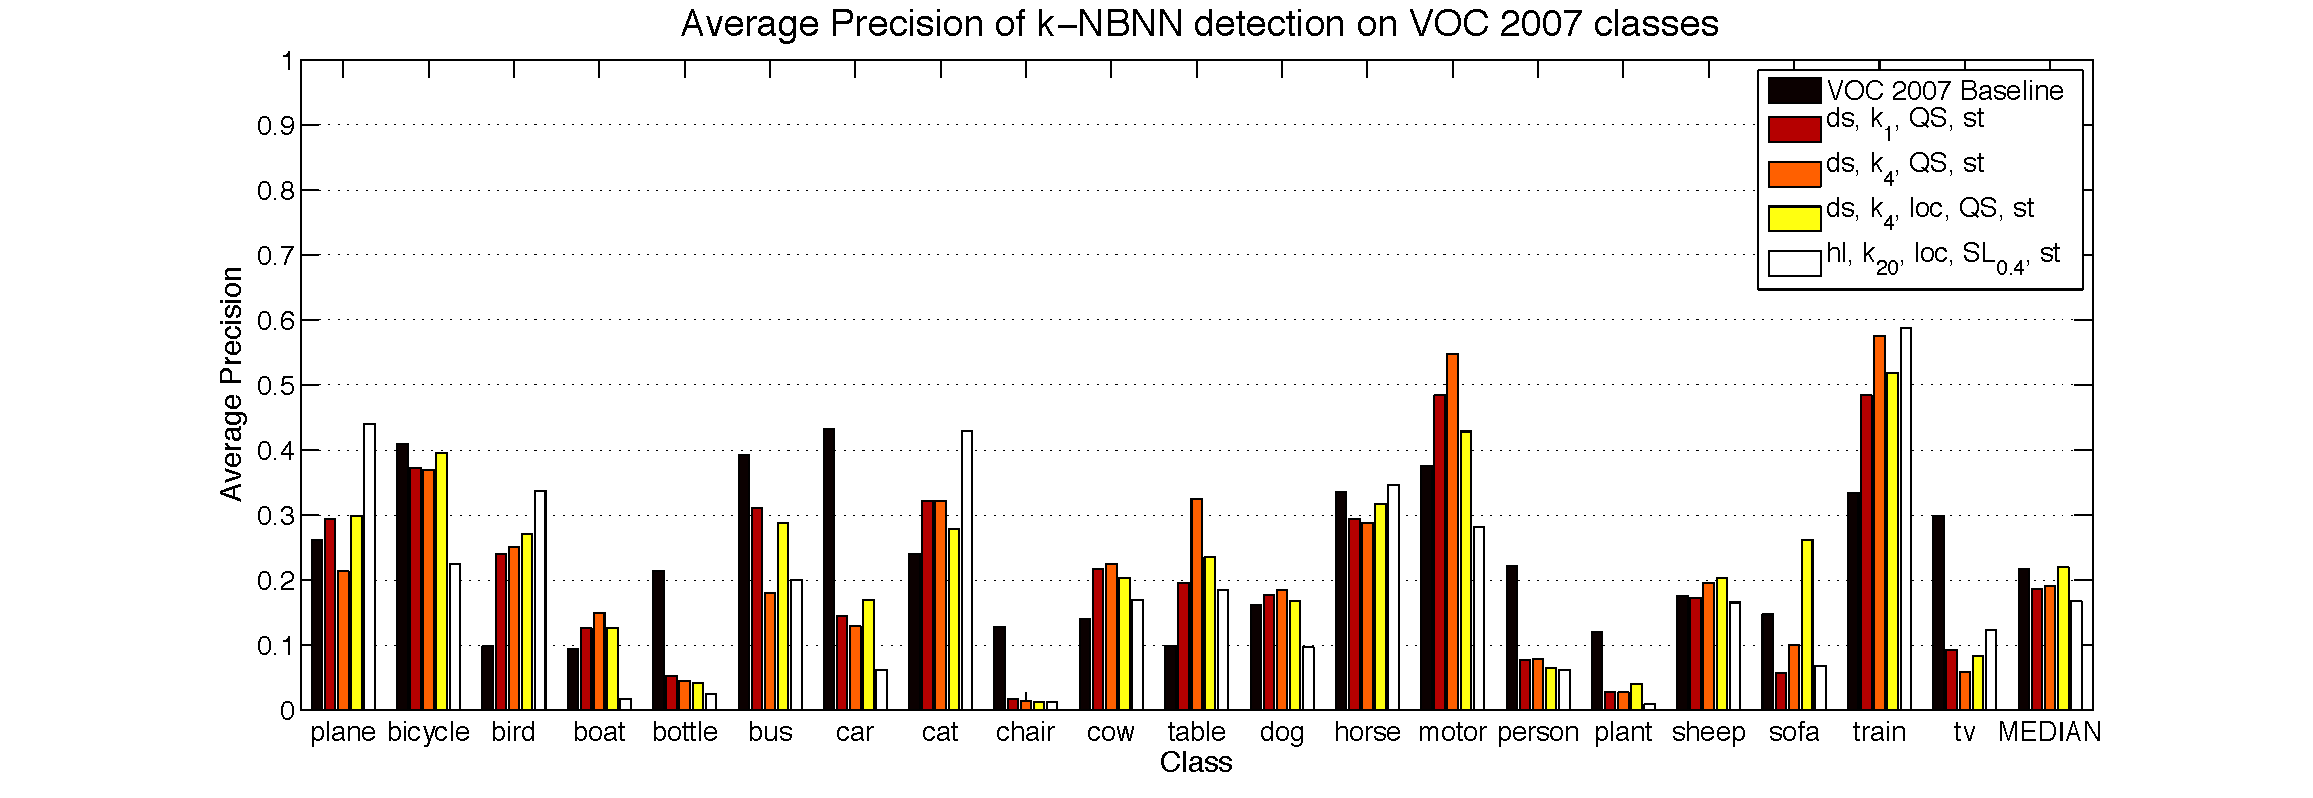
\includegraphics[width=\textwidth]{VOCklocap}
    \caption{AP for each VOC 2007 class of various tests using $k>1$, compared with both the baseline and the best results with $k=1$.}
    \label{fig:vocklocap}
\end{figure}

\begin{table}[hbt]
    \centering
    \caption{Comparison of Average Precision on the VOC 2007 test for local NBNN, and a baseline of the best performances achieved in the VOC 2007 challenge. Per class the highest three AP's are colored gold, silver, and bronze respectively.}
    \label{tab:vocallaps}
    {\footnotesize
\begin{tabular}{r|c|cccc|cc|ccc|cc}
~& \begin{sideways}VOC07 Baseline\end{sideways}& \begin{sideways}ds, $k_1$, SL$_{0.0}$, st\end{sideways}& \begin{sideways}ds, $k_1$, SL$_{0.4}$, st\end{sideways}& \begin{sideways}ds, $k_1$, QS, st\end{sideways}& \begin{sideways}hl, $k_1$, QS, st\end{sideways}& \begin{sideways}ds, $k_4$, QS, st\end{sideways}& \begin{sideways}hl, $k_4$, QS, st\end{sideways}& \begin{sideways}ds, loc, $k_4$, QS, st\end{sideways}& \begin{sideways}hl, loc, $k_4$, QS, st\end{sideways}& \begin{sideways}hl, loc, $k_{20}$, SL$_{0.4}$, st\end{sideways}& \begin{sideways}hl, $k_4$, QS, ft\end{sideways}& \begin{sideways}ds, $k_1$, SL$_{0.0}$, ft\end{sideways}\\
\hline
aeroplane&26.2&11.2&13.3&29.4&31.8&21.3&\cellBronze37.0&29.8&\cellSilver38.8&\cellGold44.0&17.5&13.7\\
bicycle&\cellGold40.9&21.8&35.7&\cellBronze37.2&18.1&37.0&12.4&\cellSilver39.6&20.3&22.5&11.8&17.3\\
bird&9.8&\cellBronze32.2&\cellSilver33.3&24.0&13.6&25.1&14.0&27.0&22.7&\cellGold33.7&5.4&7.0\\
boat&9.4&10.0&\cellSilver14.6&\cellBronze12.6&1.0&\cellGold15.0&1.6&12.6&3.2&1.7&6.2&1.9\\
bottle&\cellGold21.4&\cellBronze6.1&\cellSilver8.1&5.2&1.0&4.5&0.8&4.1&4.4&2.5&0.6&1.0\\
bus&\cellGold39.3&24.4&\cellSilver33.1&\cellBronze31.1&17.6&18.0&17.6&28.8&14.6&20.1&13.2&23.3\\
car&\cellGold43.2&14.5&\cellSilver17.7&14.5&10.9&12.9&11.6&17.0&13.6&6.1&\cellBronze17.6&15.1\\
cat&24.0&\cellGold47.1&\cellSilver46.9&32.2&33.3&32.2&33.3&27.9&27.0&\cellBronze43.0&34.2&37.5\\
chair&\cellGold12.8&0.0&\cellBronze2.0&1.7&0.7&1.4&1.8&1.2&\cellSilver2.0&1.3&1.6&0.9\\
cow&14.0&14.7&16.9&\cellSilver21.7&9.6&\cellGold22.5&10.9&\cellBronze20.4&11.8&16.9&8.0&7.2\\
diningtable&9.8&\cellSilver27.1&\cellBronze25.8&19.5&4.1&\cellGold32.5&0.7&23.5&9.1&18.4&25.3&20.9\\
dog&16.2&\cellGold26.2&\cellSilver24.3&17.6&5.3&18.5&3.9&16.8&12.6&9.6&22.9&\cellBronze23.2\\
horse&\cellSilver33.5&21.0&21.4&29.4&22.2&28.7&21.2&\cellBronze31.7&13.9&\cellGold34.7&14.6&14.9\\
motorbike&37.5&41.5&\cellSilver49.3&\cellBronze48.4&44.1&\cellGold54.7&43.4&42.8&42.6&28.1&18.1&25.2\\
person&\cellGold22.1&\cellBronze9.4&\cellSilver11.5&7.7&4.0&7.8&4.4&6.4&3.5&6.2&5.3&7.3\\
pottedplant&\cellGold12.0&0.3&1.8&\cellBronze2.7&0.4&2.7&0.2&\cellSilver4.1&0.7&0.9&1.6&0.5\\
sheep&\cellBronze17.5&12.4&15.4&17.2&16.2&\cellSilver19.6&15.5&\cellGold20.3&17.4&16.5&6.3&4.7\\
sofa&\cellSilver14.7&0.0&3.3&5.7&0.2&\cellBronze10.0&0.2&\cellGold26.2&1.1&6.8&10.0&4.4\\
train&33.4&\cellBronze52.3&48.0&48.4&48.7&\cellSilver57.6&48.5&51.9&40.5&\cellGold58.7&19.9&20.3\\
tvmonitor&\cellGold29.8&7.5&16.8&9.2&\cellSilver19.9&5.8&\cellBronze19.8&8.4&11.8&12.3&6.1&2.5\\
\hline
MEDIAN&\cellSilver21.8&14.6&17.3&18.6&12.2&\cellBronze19.0&12.0&\cellGold21.9&13.1&16.7&10.9&10.5
\end{tabular}
}
\end{table}

On the VOC test, performances are somewhat comparable to the $k=1$ experiments, as Figure~\ref{fig:vocklocap} and Table~\ref{tab:vocallaps} show. 
The methods can keep up fairly well with the baseline, but again there is much variance between classes and experiments, both in absolute performance and relative to the baseline.

Highest average performance was reached in the ``ds, loc, $k_4$, QS, st'' experiment, the median AP being 21.9\%, very slightly above the baseline. The same pattern as before emerges comparing dense sampling to harris-laplacian interest point detection: the former gets a better average precision than the latter. The results interestingly show that while the median AP's of $k$NBNN and LNBNN detection are higher than single NN detection, the differences between classes are also bigger in the new experiments. Taken over all experiments, 4 classes get highest AP using $k$NBNN, 6 classes using LNBNN and only 2 classes using single NBNN (the other 8 classes getting highest AP in the baseline). On the other hand, the second or third largest AP for most classes are among the single NBNN experiments. Experiment ``hl, loc, $k_{20}$, SL$_{0.4}$, st'' is interesting, because even though it performs mediocre on average, it scores best in 4 classes: \emph{aeroplane}, \emph{bird}, \emph{horse} and \emph{train}. Further analysis is needed to find out what causes these results.

Table~\ref{tab:vocalldurdet} shows that duration of VOC tests can get much higher for $k$NBNN and LNBNN experiments, just like the number of detections. Again, one test clearly stands out: ``ds, loc, $k_4$, QS, st''. Just like in the TUD test, this is probably caused by memory deficiency issues.

Take in mind that I trained on a subset of the available training images only, and I tested on a subset of the test set too. It would be interesting to see results on a larger train and test set, even though much of the train set was not segmented and therefore not available for comparison.

The two last experiments mentioned in Table~\ref{tab:vocalldurdet}, Table~\ref{tab:vocallaps} and the last one in Figure~\ref{fig:vocklocap}: ``hl, $k_4$, QS, ft'' and ``ds, $k_1$, SL$_{0.0}$, ft'',  were performed on the full VOC 2007 detection test set. Performance is much lower than using the smaller segmentation test set, duration and number of detections are much higher than their counterpart experiments on the smaller set. This shows some complexity issues of the method. The next section will elaborate on the possible causes and consequences of these results.

\begin{table}[hbt]
    \centering
    \caption{Test duration and total number of detections found per VOC 2007 experiment. This gives an indication of time and memory complexity.}
    \label{tab:vocalldurdet}
    \begin{tabular}{rcr}
    ~&duration (hrs)&no. of detections\\
    \hline
    ds, $k_1$, SL$_{0.0}$, st&3.27&10016\\
    ds, $k_1$, SL$_{0.4}$, st&3.39&86158\\
    ds, $k_1$, QS, st&4.30&165356\\
    hl, $k_1$, QS, st&0.95&54906\\
    ds, $k_4$, QS, st&6.39&173901\\
    hl, $k_4$, QS, st&1.00&57774\\
    ds, loc, $k_4$, QS, st&80.05&379439\\
    hl, loc, $k_4$, QS, st&2.23&159427\\
    hl, loc, $k_{20}$, SL$_{0.4}$, st&4.36&299750\\
    hl, $k_4$, QS, ft&43.49&3630083\\
    ds, $k_1$, SL$_{0.0}$, ft&72.08&231669
    \end{tabular}
\end{table}


% subsubsection lnbnn_results (end)
% section local_nbnn_detection (end)
% chapter experimental_setup (end)